\chapter{Implementação e Avaliação}
\label{cha:Implementação e Avaliação}


Nesse capítulo serão abordados todas as etapas da processamento, criação/treinamento e avaliação dos 3 modelos selecionados. Na etapa de treinamento será explicado um pouco do processamento das imagens, na fase criação/treinamento será exemplificado melhor o padrão de construção dos modelos e, por fim, na fase de avaliação serão exibidos os resultados encontrados.

\section{Análise e Processamento dos Dados}

Como apontado no capítulo \ref{cha:Projeto e Especificação do Sistema}, o dataset consiste numa série de imagens de raio-X de pulmões. As imagens têm extensão \verb|.jpeg|, não possuem um tamanho fixo e estão separadas em 3 pastas (\verb|train|, \verb|test| e \verb|val|) de acordo com suas devidas funções. Por isso, antes de começar o treinamento e avaliação dos modelos de rede neural, foi necessário passar por uma etapa de processamento, onde realizaremos transformações no conjunto de dados, seguindo o algorítmo \ref{alg:processamentoDados}.

\begin{algorithm}
    \DontPrintSemicolon
    \KwIn{Caminho de dados}
    \KwOut{Vetor com dados carregados}
    \BlankLine
    \emph{resultado $\xleftarrow{}$ cria\_lista\_vazia()}\;
    \ForAll{classe} {
        \emph{caminho $\xleftarrow{}$ monta\_caminho(Caminho de dados, classe)}\;
        \emph{acessa\_caminho(caminho)}\;
        \ForAll{imagem}{
            \emph{carrega\_imagem()}\;
            \emph{redimensiona\_imagem()}\;
            \emph{atualiza\_vetor(resultado, [imagem, classe])}\;
        }
    }
    \emph{Retorna resultado}\;
    
    \caption{Processamento dos dados}
    \label{alg:processamentoDados}
\end{algorithm}\DecMargin{1em}

O algorítmo \ref{alg:processamentoDados} recebe de entrada um diretório onde ele deverá ler as imagens e retorna um vetor com as imagens carregadas. Esse algorítmo será executado para todos os 3 diretórios (\verb|train|, \verb|test| e \verb|val|), onde ele percorrerá por todas as imagens redimensionando para o tamanho ideal (nesse caso sendo 150 pixels por 150 pixels). Por fim ele atualiza o vetor de saída com um novo vetor contendo a imagem transformada e sua classe (NORMAL ou PNEUMONIA).

Utilizando a função criada, podemos carregar as imagens para 3 cenários diferentes (\verb|train|, \verb|test| e \verb|val|) e analiser o conjunto. Um exemplo de imagens lidas aplicando a paleta de cores \verb|bone| está representada na imagen \ref{pic:3x3_raiox}.

\begin{figure}[!ht]
    \begin{center}
    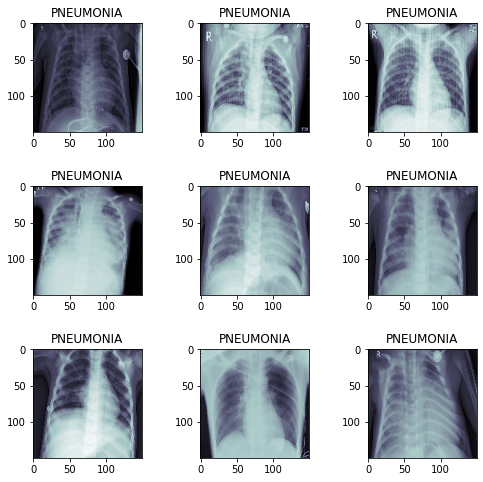
\includegraphics[width=350pt]{pictures/images_chest.png}
    \caption{Raio-X de pulmões}
    \label{pic:3x3_raiox}
    \end{center}
\end{figure}

Colocando as imagens em um dataframe da bilbioteca pandas, conseguimos ter uma visualização melhor e exibir gráficos envolvendo a quantidade de cada classe em cada estágio do processo. 

Na imagem \ref{pic:estagios_treinamento}, é trivial perceber que as classes  estão desbalanceadas no conjunto de dados, onde a barra vermelha representa as imagens de pulmões com pneumonia e a barra azul de pulmões saudáveis, tendo seus estágios de treino, teste e validação representando 89\%, 10\% e  0.2\% da base respectivamente. Sendo assim, será necessário aplicar uma etapa de enriquecimento de dados (\textit{data augmentation}) para gerar novas amostras para cada estágio.

\begin{figure}[!ht]
    \begin{center}
    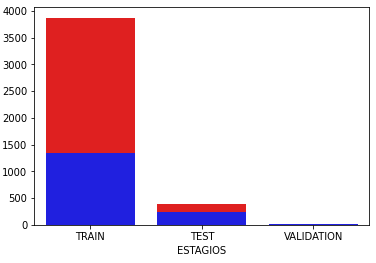
\includegraphics[width=300pt]{pictures/dados_estagios.png}
    \caption{Dados dos estágios}
    \label{pic:estagios_treinamento}
    \end{center}
\end{figure}

\newpage
Para seguir com o passo do enriquecimento de dados, utilizamos uma função da biblioteca \verb|keras| chamada de \verb|ImageDataGenerator| que aceita uma série de parâmetros para gerar diferentes variações nas imagens. Para o treinamento e validação do modelo foram utilizados diferentes configurações:

\begin{enumerate}
    \item As imagens foram rotacionadas em 30º, sendo útil para reconhecer objetos que podem aparecer em várias orientações.
    \item As imagens foram transladadas ligeiramente para cima e para lado em 10\% do seu valor, com o objetivo de reconhecer traços de pneumonia mesmo não estando centralizado na imagem
    \item Um zoom de 20\% foi aplicado tendo como finalidade reconhecer objetos de diferentes escalas.
    \item Um \textit{flip} horizontal, já que a orientação horizontal do raio-X não importa. Nesse caso, não tem problema trocar pulmões esquerdos por direitos, pois o objetivo do modelo é puramente binário.
\end{enumerate}

Outra alteração necessária a ser feita foi a normalização dos valores dos pixels. Nas imagens atuais, os valores de cores estão entre 1 e 255, porém um modelo de CNN performa melhor se essa grandeza estiver entre 0 e 1. 
\newpage 

\section{Criação dos Modelos}

Uma função específica foi desenvolvida para construir e treinar modelos seguindo um formato padrão. Utiliza-se a função Sequential da biblioteca keras para definir o modelo, sobre a qual são empilhadas diversas camadas necessárias. Estas podem incluir convoluções, operações de \textit{pooling}, normalizações, entre outras. Todas as funções empregadas na criação dos modelos aderem a este padrão estabelecido exemplificado no algorítmo \ref{alg:criacaoModelo}


\begin{algorithm}
\DontPrintSemicolon
\KwIn{Número de épocas, tamanho do lote, dados de treino e dados de validação}
\KwOut{Histórico de treinamento e modelo treinado}
\BlankLine
\emph{modelo $\xleftarrow{}$ Sequential}\;
\emph{modelo.empilha\_camadas\_necessárias()}\;
\emph{modelo.compilar(otimizador=otimizador\_escolhido)}\;
\emph{histórico $\xleftarrow{}$ modelo.treinar(dados de treino, dados de validação, número de epocas, tamanho do lote)}\;
\emph{Retorna histórico, modelo}
\caption{Criação e treinamento de um modelo}\label{alg:criacaoModelo}
\end{algorithm}\DecMargin{1em}

Como especificado na \ref{cha:Pesquisas Realizadas}, os algorítmos de rede neural ResNet50 e InceptionV3, foram treinados com imagens com 3 canais de cores. No caso do \textit{dataset} utilizado, não será necessário aplicar técnica alguma para "colorir" as imagens de escala cinza, basta apenas repetir a mesma camada cinza 3 vezes ao enviar as imagens para o modelo. 


\section{Resultados}

Depois de treinar os modelos, avaliamos sua eficácia usando várias métricas, incluindo acurácia, perda durante as fases de treinamento e teste, matrizes de confusão e relatórios de classificação. Experimentos variados foram realizados, empregando otimizadores como \textbf{Adam} e \textbf{RMSProp} em combinação com modelos como InceptionV3, ResNet50, e uma rede neural convolucional. Os treinamentos foram realizados com 20 épocas, gerando os resultados encontrados na tabela \ref{tab:resultados_tabela}.
\newpage

\begin{table}[!h]
    \centering
    \renewcommand{\arraystretch}{1.5} % Aumenta o espaçamento entre as linhas
    \begin{tabular}{c|c|c|c|c|c|c|c}
       Modelo  & Otimizador & Precisão & Perda & Acurácia & f1-score & Recall & Miss \\
         \hline  
        CNN & RMSProp & 0.88 & 0.54 & 87.82\% & 0.88 & 0.88 & 76 \\
        ResNet50 & RMSProp & 0.91 & 0.23 & 90.86\% & 0.91 & 0.91 & 57\\ 
        InceptionV3 & RMSProp & 0.94 & 0.15 & 94.23 \% & 0.94 & 0.94 & 36 \\
        CNN & Adam & 0.89 & 0.27& 88.94\% &  0.89 &  0.89 & 69 \\
        ResNet50 & Adam & 0.93 & 0.17 & 93.42\% & 0.93 & 0.93 & 41 \\
        \cellcolor{green!25}InceptionV3 & \cellcolor{green!25}Adam & \cellcolor{green!25}0.95 &  \cellcolor{green!25}0.16 &  \cellcolor{green!25}95.19\% & \cellcolor{green!25}0.95 & \cellcolor{green!25}0.95 &  \cellcolor{green!25}30  
    \end{tabular}
    \caption{Resultados do treinamento}
    \label{tab:resultados_tabela}
\end{table}

A precisão é determinada pela proporção de predições acertadas para uma determinada classe em relação ao total de predições feitas para essa classe. Já o recall mede a proporção de predições acertadas para uma classe em comparação com o número total de casos verdadeiros dessa classe no conjunto de dados. O F1-Score, por sua vez, é calculado como a média harmônica da precisão e do recall, resultando em uma métrica única que balanceia as duas. Depois de calcular essas métricas para cada classe, realiza-se uma média delas para chegar aos valores apresentados na tabela.

Analisando mais detalhadamente a tabela \ref{tab:resultados_tabela} é perceptível que, quando foi feita a troca do otimizador RMSProp para Adam tivemos um aumento de até 2 pontos percentuais na acurácia, recall, f1-score e precisão, assim como a queda nesse caso, bem mais significativa, da perda. Ambos cenários indicam resultado positivos para esse dataset.

\begin{figure}[!ht]
    \begin{center}
    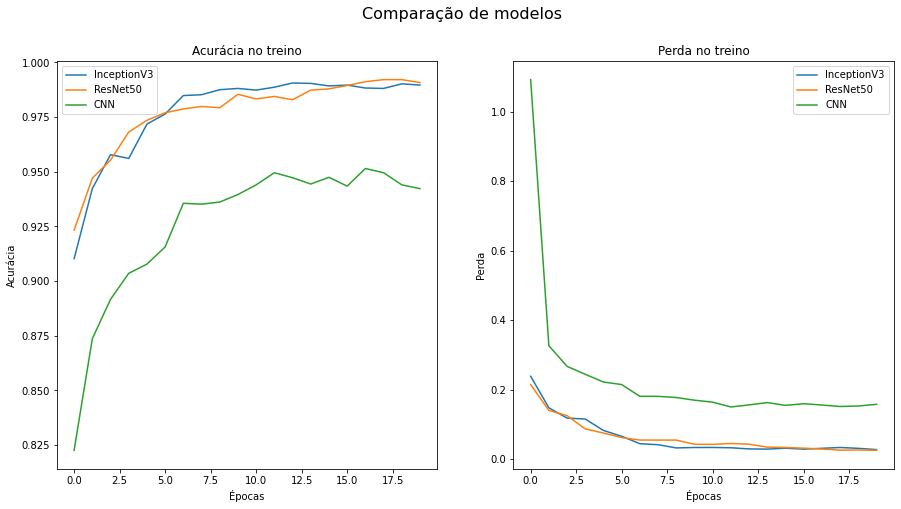
\includegraphics[width=400pt]{pictures/comparação entre modelos.png}
    \caption{Comparação de acurácia e perda}
    \label{pic:grafico_comparativo}
    \end{center}
\end{figure}

\newpage 

Analisando a imgem \ref{pic:grafico_comparativo}, percebemos que a curva da CNN se distancia das outras, mantendo uma acurácia menor e uma perda maior. Isso se dá devido ao nível de simplicidade e à ausência de pesos pré-treinados, como é o caso da InceptionV3 e da ResNet50. Falando um pouco sobre esses dois últimos modelos, é notável que ambos ficam muito próximos tanto no quesito de minimizar a perda quanto a maximizar a acurácia. De um modo geral, a rede neural InceptionV3 se sai melhor do que a ResNet50, pelo fato de convergir para seus valores ideais de maneira mais "rápida".

Analisando as matrizes de confusão para cada um dos modelos, são notados alguns resultados interessantes:

\begin{table}[!ht]
    \centering
    \begin{tabular}{l|l|c|c|c}
        \multicolumn{2}{c}{}&\multicolumn{2}{c}{Valor previsto}&\\
        \cline{3-4}
        \multicolumn{2}{c|}{}&Pneumonia&Normal&\multicolumn{1}{c}{Total}\\
        \cline{2-4}
        \multirow{2}{*}{Valor real}& Pneumonia & $356$ & $34$ & $390$\\
        \cline{2-4}
        & Normal & $35$ & $199$ & $234$\\
        \cline{2-4}
        \multicolumn{1}{c}{} & \multicolumn{1}{c}{Total} & \multicolumn{1}{c}{$391$} & \multicolumn{    1}{c}{$233$} & \multicolumn{1}{c}{$624$}\\
    \end{tabular}
    \caption{CNN - Matriz de confusão}
    \label{tab:cm_cnn}
\end{table}


Para os resultados previstos incorretamente, o pior caso, seriam os falsos positivos. Na CNN genérica montada eles representam aproximadamente 5.4\% do total de previsões, como mostra a tabela \ref{tab:cm_cnn}.

\newpage

\begin{table}[!ht]
    \centering
    \begin{tabular}{l|l|c|c|c}
        \multicolumn{2}{c}{}&\multicolumn{2}{c}{Valor previsto}&\\
        \cline{3-4}
        \multicolumn{2}{c|}{}&Pneumonia&Normal&\multicolumn{1}{c}{Total}\\
        \cline{2-4}
        \multirow{2}{*}{Valor real}& Pneumonia & $373$ & $17$ & $390$\\
        \cline{2-4}
        & Normal & $24$ & $210$ & $234$\\
        \cline{2-4}
        \multicolumn{1}{c}{} & \multicolumn{1}{c}{Total} & \multicolumn{1}{c}{$397$} & \multicolumn{    1}{c}{$227$} & \multicolumn{1}{c}{$624$}\\
    \end{tabular}
    \caption{ResNet50 - Matriz de confusão}
    \label{tab:res_cm}
\end{table}

Implementando um modelo mais robusto, é notória a diferença, representada na tabela \ref{tab:res_cm}, em ambos os casos incorretos com falsos positivos caindo 50\% e falsos negativos caindo 25\%.

\begin{table}[!ht]
    \centering
    \begin{tabular}{l|l|c|c|c}
        \multicolumn{2}{c}{}&\multicolumn{2}{c}{Valor previsto}&\\
        \cline{3-4}
        \multicolumn{2}{c|}{}&Pneumonia&Normal&\multicolumn{1}{c}{Total}\\
        \cline{2-4}
        \multirow{2}{*}{Valor real}& Pneumonia & $382$ & $8$ & $390$\\
        \cline{2-4}
        & Normal & $22$ & $212$ & $234$\\
        \cline{2-4}
        \multicolumn{1}{c}{} & \multicolumn{1}{c}{Total} & \multicolumn{1}{c}{$404$} & \multicolumn{    1}{c}{$220$} & \multicolumn{1}{c}{$624$}\\
    \end{tabular}
    \caption{InceptionV3 - Matriz de confusão}
    \label{tab:cm_incep}
\end{table}

Por fim, no InceptionV3 são encontrados os menores valores de classificações incorretas em todo o teste. Podemos ver na tabela \ref{tab:cm_incep} que, o total de falsos positivos decresceu 76\% em relação ao valor original, e os falsos negativos, um total de 37\%.

Com base no que foi apresentado, fica evidente que o modelo InceptionV3 supera os demais em eficácia, otimizando a precisão e reduzindo significativamente as perdas. Esse modelo se destaca especialmente na matriz de confusão ao registrar o menor número de falsos positivos e negativos. Essa característica é crucial, particularmente em análises médicas de doenças, onde um resultado falso negativo pode ter consequências graves para a saúde do paciente. Portanto, a eficiência do InceptionV3 em minimizar esses erros contribui diretamente para a confiabilidade e segurança dos diagnósticos.
